% Implementation
\section{Implementation}

\subsection{Starten der App}
Beim Starten der App wird duch mehrere Entscheidungen festgelegt, welche Maske dem Benutzer angezeigt wird. In Abbildung \ref{image-kort-startup-activitydiagram} ist der Ablauf grob dargestellt.

\begin{figure}[H]
	\centering
	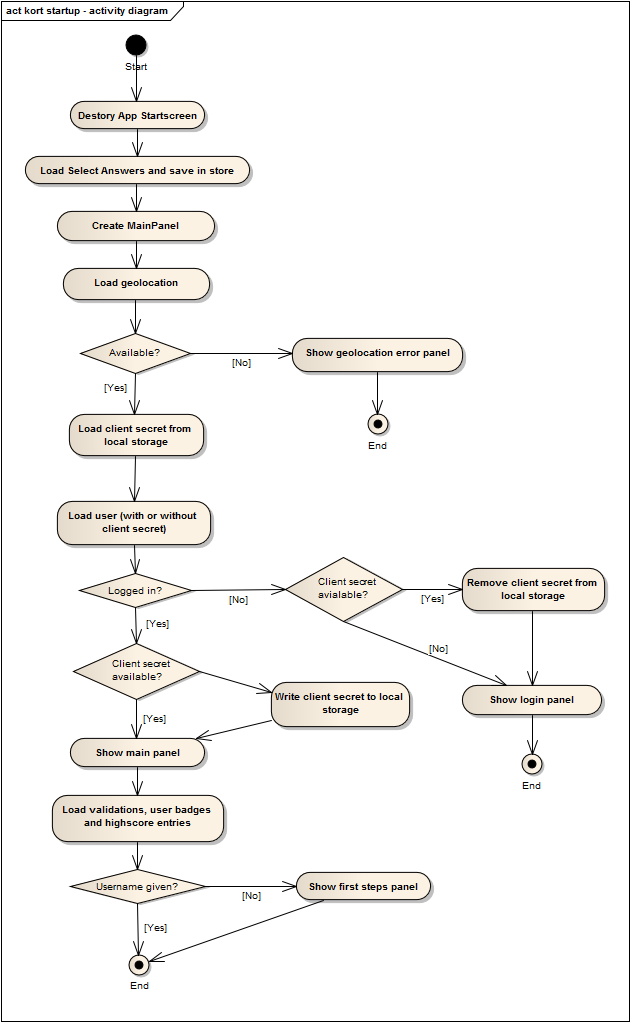
\includegraphics[scale=0.55]{images/uml/kort-startup-activitydiagram}
	\caption{Ablauf beim Starten der App}
	\label{image-kort-startup-activitydiagram}
\end{figure}

Schlussendlich wird dem Benutzer eine der folgenden Masken angezeigt:

\begin{itemize}
\item \textbf{Geolocation Fehler Maske}: Wenn Geolocation nicht gelesen werden kann.
\item \textbf{Login Maske}: Wenn Benutzer noch nicht eingeloggt ist
\item \textbf{Erste Schritte Maske}: Wenn Benutzer noch keinen Benutzernamen gewählt hat
\item \textbf{Hauptmaske}: Wenn der Benutzer bereit ist, die App zu benutzen
\end{itemize}

\subsection{Sencha Cmd}
\label{sencha-cmd}
Das Grundgerüst der App wurde komplett mit dem Sencha-eigenen Build-Tool \emph{Sencha Cmd 3.0.0}\footnote{\url{http://www.sencha.com/products/sencha-cmd}} generiert.
Dieses bietet verschiedene Build-Möglichkeiten an:

\begin{table}[H]
\centering
\begin{tabular}{|p{0.2\twocelltabwidth}|p{0.8\twocelltabwidth}|}
\hline
\textbf{Build} & \textbf{Beschreibung} \\
\hline
testing & Bei diesem Build werden die JavaScript-Quelldateien in einer Datei zusammengefasst. Zusätzlich werden lediglich die verwendeten Dateien kopiert. \\
\hline
production & Der Production-Build entspricht grundsätzlich dem Testing-Build. Zusätzlich werden aber noch die JavaScript-Quelldateien komprimiert. \\
\hline
package/native & Mit diesen Builds lassen sich native Apps für die verschiedenen mobilen Betriebssysteme generieren. \\
\hline
\end{tabular}
\caption{Verschiedene Build-Möglichkeiten mit Sencha Cmd}
\label{table-sencha-cmd-build}
\end{table}

Durch den Einsatz von Sencha Cmd wird es möglich mit einem geringen Mehraufwand, eine native App zu generieren und diese in den verschiedenen App-Stores (Apples AppStore, Google Play Store) anzubieten.

\subsubsection{Konfiguration}
Der Buildprozess wird in der Datei \inlinecode{app.json} konfiguriert.

\begin{table}[H]
\centering
\begin{tabular}{|p{0.2\twocelltabwidth}|p{0.8\twocelltabwidth}|}
\hline
\textbf{Property} & \textbf{Beschreibung} \\
\hline
\inlinecode{"js"} & Hier können die JavaScript-Quelldateien, welche von der App verwendet werden eingetragen werden. Diese werden im Buildprozess automatisch in den \inlinecode{<head>}-Bereich des \inlinecode{index.html}-Files geschrieben. \\
\hline
\inlinecode{"css"} & Ähnlich wie das \inlinecode{"js"}-Property nur für CSS-Ressourcen. \\
\hline
\inlinecode{"ressources"} & Hier können weitere Ressourcen wie Grafiken oder Libraries angegeben werden. \\
\hline
\end{tabular}
\caption{Wichtige Konfigurations-Eigenschaften in Sencha Cmd (app.json)}
\label{table-sencha-cmd-appjson}
\end{table}

Zusätzlich ist in der Datei \inlinecode{.sencha/app/sencha.cfg} der Classpath für die App definiert.

Weitere Informationen zur Konfiguration findet man im entsprechendem Guide der Sencha Docs\footnote{\url{http://docs.sencha.com/touch/2-1/\#!/guide/command\_app}}.

\subsubsection{App Build starten}
Zur Erstellung eines \textsc{Kort}-Builds muss \emph{Sencha Cmd} in der Version 3.0.0.250 installiert sein.
Der Build kann von der Konsole aus gestartet werden. Dazu muss in das Root-Verzeichnis von \textsc{Kort} gewechselt werden und folgender Befehl eingegeben werden:

\inlinecode{sencha app build <environment>}

Die erstellt App wird dann in dem entsprechenden Verzeichnis abgelegt:

\inlinecode{/build/Kort/<environment>}

\subsection{Internernationalisierung (i18n)}
\label{i18n}
Die Oberfläche von \textsc{Kort} wurde bereits für eine mögliche Übersetzung vorbereitet.
Dazu wurde das Plugin \emph{Ext.i18n.Bundle-touch}\footnote{\url{https://github.com/elmasse/Ext.i18n.Bundle-touch}} für Sencha Touch eingesetzt. Dieses ermöglicht es einzelne Texte in externen Sprach-Property-Files auszulagern.

Bei \textsc{Kort} befinden sich diese Files im Verzeichnis \inlinecode{/resources/i18n/} und müssen nach folgendem Schema benannt werden: \inlinecode{Kort\_<locale>.props}.
Die verwendete Sprache ist in der Funktion \inlinecode{prepareI18n()} der Datei \inlinecode{app.js} festgelegt.

\lstset{language=JavaScript}
\begin{lstlisting}[caption=kort - Sprache definieren, label=kort-choose-language]
prepareI18n: function() {
	Ext.i18n.Bundle.configure({
		bundle: 'Kort',
		language: 'de-CH',
		path: 'resources/i18n',
		noCache: true
	});
}
\end{lstlisting}

Hier kann über das \inlinecode{language}-Property die Sprache konfiguriert werden.
Falls das Property weggelassen wird, wird die aktuelle Spracheinstellung des Browsers verwendet.
Wird dabei die entsprechende Datei nicht gefunden, verwendet das Plugin die Datei \inlinecode{Kort.props}.